\section{Control a Physical Toy Rover with AutoFOCUS3}
\label{sec:toy_rover_controller}

We have been offering the practical course "From Sensors to Driving Functions - Develop Your Own Car" at the Technical University of Munich in the past year. The students are provided with the requirements to model a system, from the logical architecture to the platform architecture, using \af. Then the code is generated which is executed on the hardware.  We provide the students with the rovers and fix any bugs found by them in \af. Additionally, students are also required to integrate the modeled system running on Raspberry Pis with the actual rover hardware, i.e., instead of using a joy stick, the developed system controls the rover.

The model used in this case study was developed by the students of this practical course in the summer semester 2018. We have taken this model and reused the elements relevant to this case study. 

The goal of the practical course was to implement platooning for rovers. Rovers were expected to drive in a platoon following the one ahead while maintaining only a small safety distance. Capability to follow another rover is a necessary feature required for implementing platooning. For this case study we have reused and extended the components dealing with this feature. 

We now briefly describe the complete system developed during the course. The students were divided in four teams each dealing with a specific part of the development: platooning, lane keeping, communication and simulation.

\subsection{Platooning}
The platooning team was responsible for developing the logical aspect of the platooning system. The functionality was divided into following sub-features: platooning as leader, platooning as follower, create platoon, fuse platoons, split platoon and leave platoon.

The team was provided with the model containing basic features (which were developed by the students of the previous practical course) like emergency braking, adaptive cruise control and were supposed to further develop this model providing the platooning feature.

\begin{figure*}[!h]
	\centering
	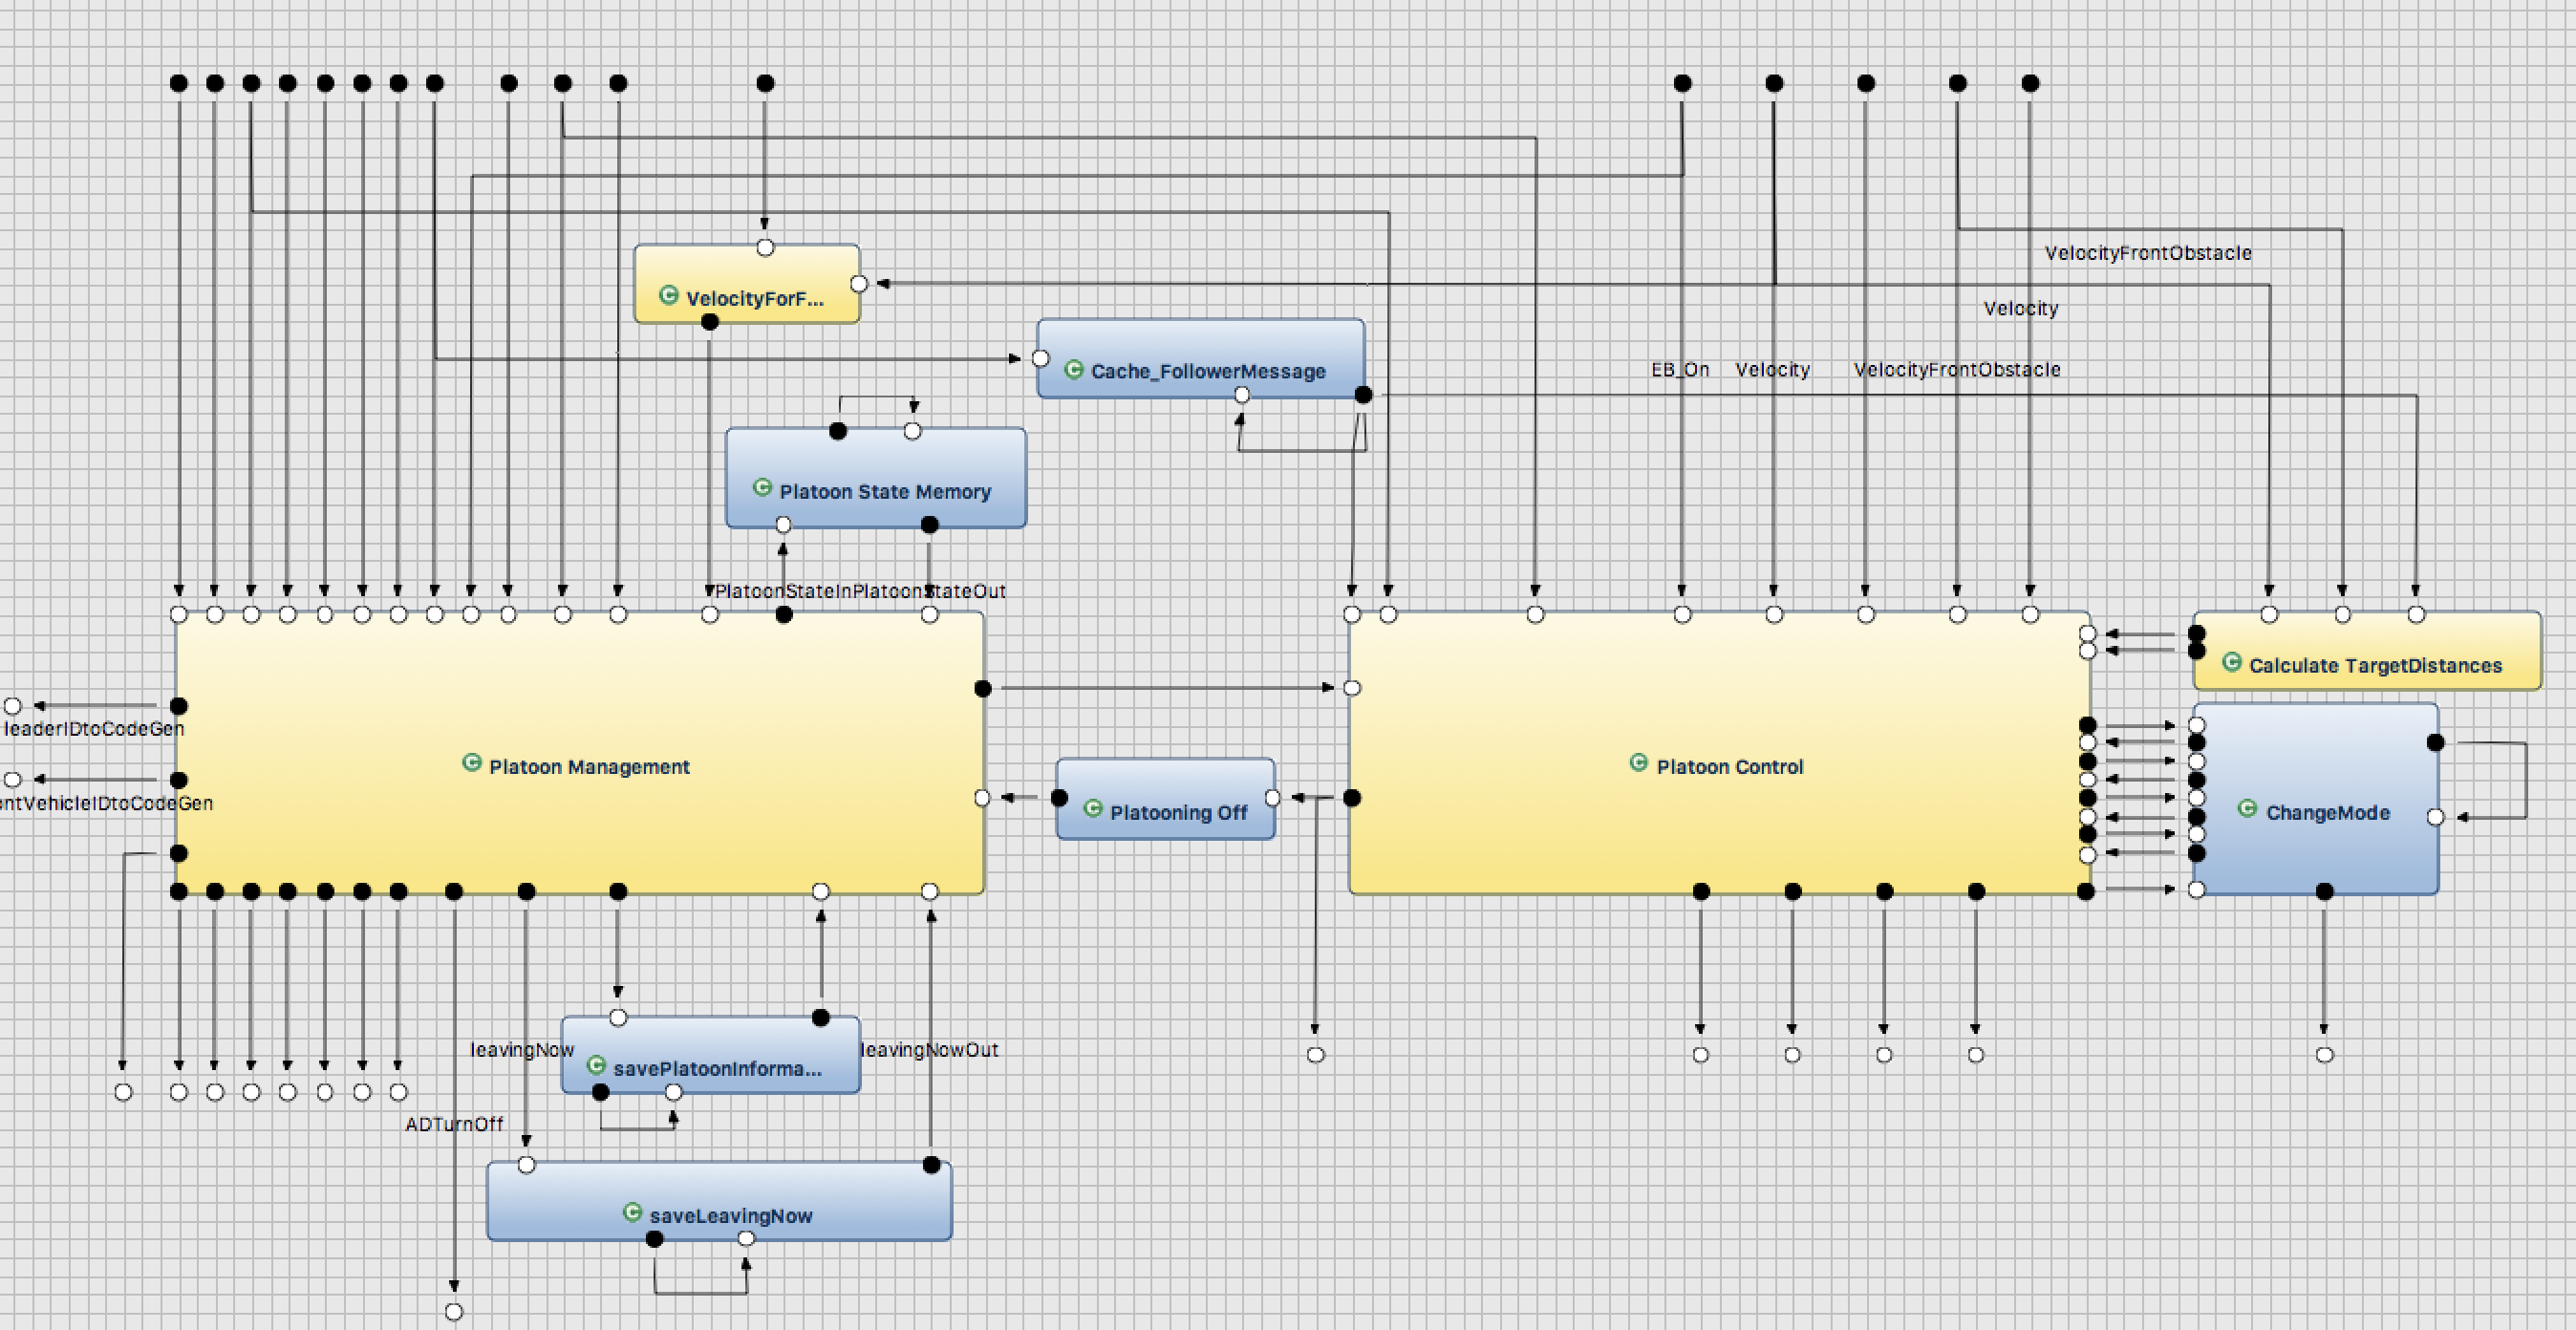
\includegraphics[width=1\textwidth]{./img/platooningArchitecture.png}
	\caption{Platooning architecture}
	\label{fig:platooning}
\end{figure*}

Figure \ref{fig:platooning} shows the architecture of the platooning component. There are two main components: platoon management and platoon control. The control component controls the behavior of each platoon member ensuring that the whole platoon moves as a single vehicle. It is responsible for vehicles to move at the constant speed, brake and accelerate simultaneously. It takes input from the sensor data, processes it and outputs driving signals such as target velocity and steering angle. The management component is responsible for processing platoon messages (e.g., joining, splitting, leaving the platoon), handling internal platoon states, and communication with the platoon control component.
 
\subsection{Lane keeping}
The lane keeping team was responsible for keeping the rover in the same lane while driving. The team mounted a camera on the rover. This image was then processed on a dedicated Raspberry Pi to detect the lane and map it on the world coordinate system (relative to the center of the rover's front-bumper). The lane-data thus generated is delivered using TCP to the system that was modeled using \af. The system then calculates the required steering angle to stay in the lane based on this data and sends out the control signal to turn the steering accordingly. Figure \ref{fig:lane_keeping} shows the controller architecture for lane keeping as modeled in \af. 

\begin{figure*}[!h]
	\centering
	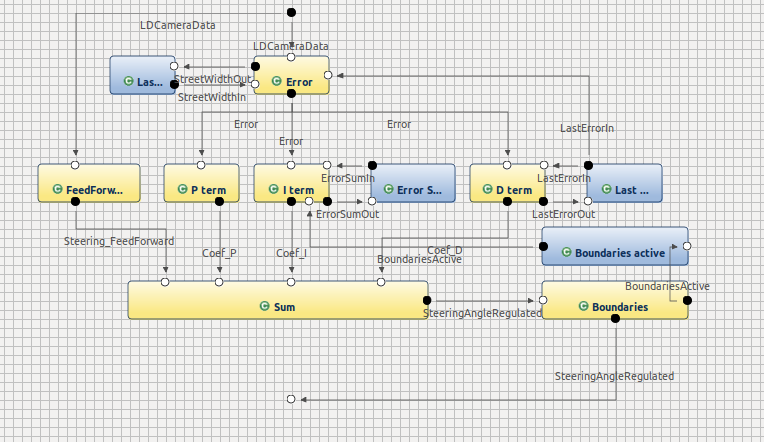
\includegraphics[width=1\textwidth]{./img/LK_Controller_Screenshot.png}
	\caption{Controller for lane keeping}
	\label{fig:lane_keeping}
\end{figure*}


\subsection{Communication}

The communication team was responsible for: 
\begin{enumerate}
	\item \textit{Intra vehicle communication}: Setting up a CAN-communication between multiple Raspberry Pis on the same rover.
	\item \textit{Inter vehicle communication}: Developing a mechanism for communication between rovers using wifi. This communication uses UDP broadcasts.
	\item \textit{Control center}:  Developing a debugging tool which can be used to intercept and modify messages between the system and the rover, e.g. sensor data, or steering command.
\end{enumerate}

\subsection{Simulation}

The simulation team was responsible for conducting hardware in the loop tests to assist in the development of the system. The team used the software CarMaker \footnote{https://ipg-automotive.com/products-services/simulation-software/carmaker/} to create a vehicle data set. CarMaker and AF3 both support functional mock-up interface (FMI) \footnote{https://fmi-standard.org}. AF3 model was exported as FMU and imported in CarMaker for to be cosimulated with the designed vehicle.

\begin{figure*}[!h]
	\centering
	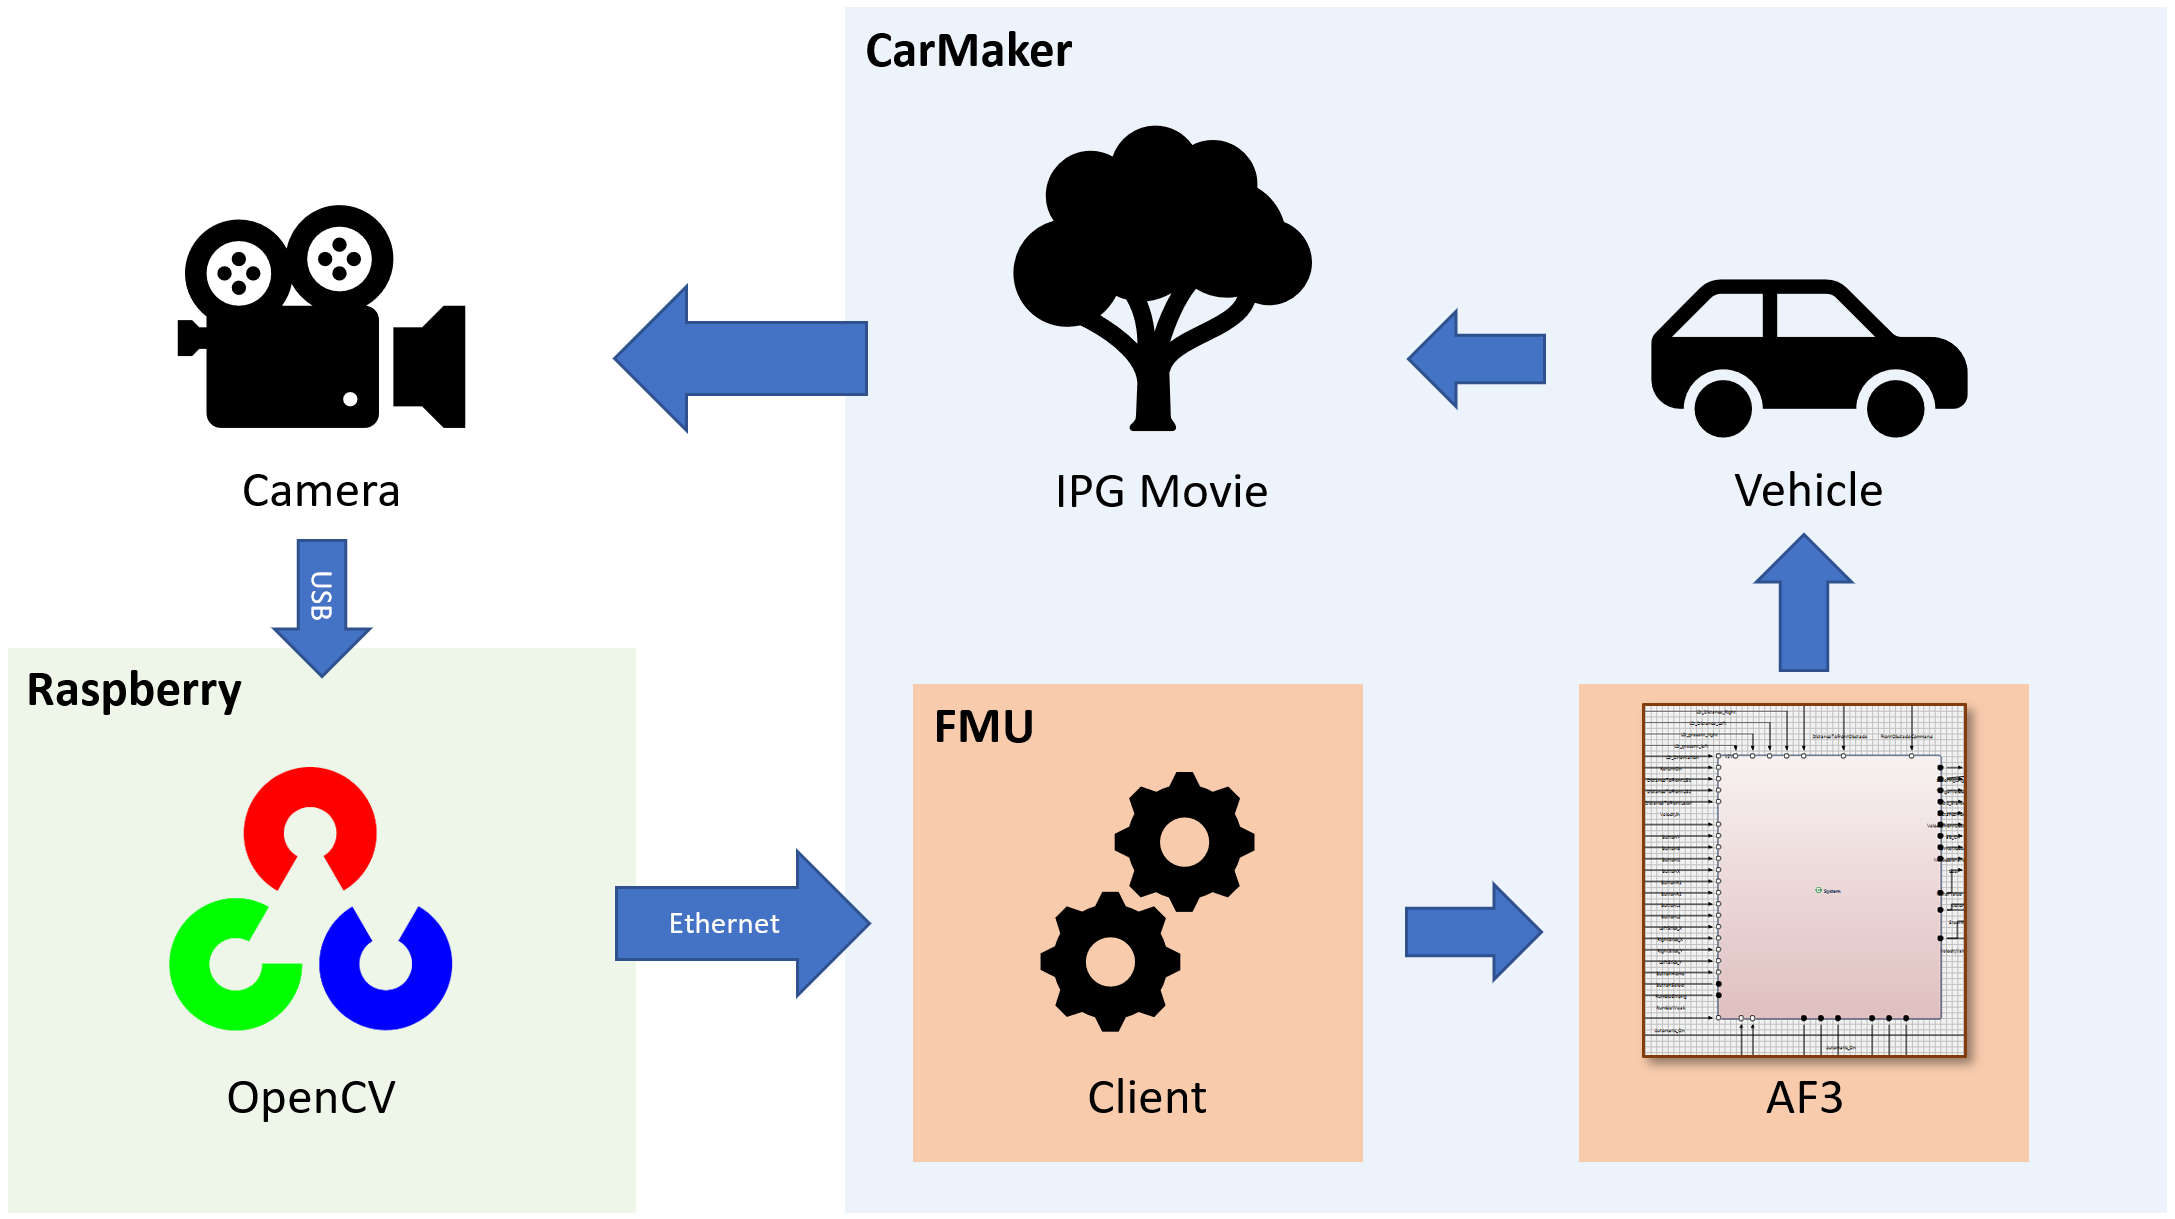
\includegraphics[width=1\textwidth]{./img/lk_concept.png}
	\caption{The simulation panel of \af}
	\label{fig:simulation}
\end{figure*}


